\documentclass[a4paper,10pt]{article}
\usepackage{fullpage}
\usepackage{times}
\usepackage{hyperref}
\usepackage{graphicx}
\graphicspath{ {./images/} }
\usepackage{multirow}
\graphicspath{ {./images/} }


\begin{document}

\title{EDI: Third Lab Report}
%Insert your name and ID inside the brackets
\author{Aiman Al Masoud - 502044}
\date{\today}

\maketitle

\begin{abstract}
%Insert a short summary of your lab activities.
\end{abstract}

\clearpage
\clearpage
\clearpage
\clearpage
\clearpage

\setcounter{page}{1}
%Figures and tables must be cited in the text and explained in detail.

\section{Parallel Connections}
% 

Page Load Time (PLT) is one of the most critical performance evaluation metrics for a website, as it correlates directly to user experience. 

PLT takes into account both the time to download the html of a page, as well as the time to download all of its embedded objects, as a browser would typically do when directed to navigate to a page.

An acceptable Page Load Time for a website in 2022 ranges between 1 and 2 seconds, but it depends on the context, and having an even lower Page Load Time is desirable; users obviously tend to abandon websites that take more time to load than their competitors. [\ref{article1}] 


\subsection{Firefox's About Config}

The first experiment that was performed, pertains to the effect of parallel TCP connections on Page Load Time. As power users will know, modern web browsers allow them to peek into various configuration settings and tweak them, this is especially true of Mozilla Firefox, where the user can access various technical settings by typing in 'about:config' into the navigation bar, and hitting enter. 

More specifically, one of these configuration parameters is called 'network.http.max-persistent-connections-per-server', and, as the name suggests, it governs the maximum amount of concurrent persistent TCP connections that the browser is allowed to sustain at a time, with any particular web server over the Internet. [\ref{article2}] 

By default, the value for this option is set to '6', but it can be changed. Does decreasing it or increasing it have an effect on PLT? Do higher values of this parameter lead to performance improvements when loading pages? 

\subsection{HTTP/1 vs HTTP/2}

Here comes to play an important distinction between websites, and that is difference between websites running on HTTP/1 and HTTP/2: the first two major versions of the ubiquitous Hypertext Transfer Protocol. 

There are various ways in which HTTP/2 tried to improve on HTTP/1, but what is of specific interest to us in this particular inquiry is that: websites running on HTTP/1 tend to favor connections to multiple separate servers, to download the objects of a page in parallel, and overcome the limitation imposed by browsers on the number of parallel connections to a single server, a technique known as Domain Sharding [\ref{article3}]. 

HTTP/2 helped overcome this very necessity, by introducing Streams that could convey multiple
concurrent (and bi-directional) HTTP requests within a single persistent TCP connection; thus eliminating the need to connect to separate resource servers, and even eliminating the overhead associated to having to open multiple TCP connections with them. This is something that, at least on the long run, will render the technique of Domain Sharding obsolete [\ref{article3}].

So, to go back to the original question: resource intensive HTTP/1 websites may benefit from an increased number of parallel TCP connections, as they only support a single HTTP request per TCP connection. On the other hand, HTTP/2 websites support multiple concurrent HTTP requests over the same TCP connection, hence, from a theoritical viewpoint, it shouldn't make much of a difference to them if the client allows them to open multiple TCP connections.


\subsection{Methodology and experimental setup}

The experiment was performed in practice, by measuring the PLTs of 6 different websites (3 HTTP/1 and 3 HTTP/2 websites) under two different conditions: 1 and 6 maximum connections per server.

The browser that was employed for the experiment was Firefox, and the number of maximum connections was set tweaking the aforementioned: "network.http.max-persistent-connections-per-server" parameter.

Although the experiment summarized in table 1 isn't exhaustive, it clearly shows that HTTP/1 websites fare much better when granted a higher number of connections per sever. 

\clearpage

\begin{table}[h!]
\centering
\begin{tabular}{|c|c|l|}
\hline
\multicolumn{1}{|r|}{\textbf{}} & \multicolumn{1}{l|}{} & \textbf{Average PLT (seconds)}         \\ \hline
\textbf{HTTP Version}          & \textbf{Connections}  & \multicolumn{1}{c|}{\textbf{}} \\ \hline
\multirow{2}{*}{\textbf{1}}     & \textbf{1}            & 3.017778                       \\ \cline{2-3} 
                                & \textbf{6}            & 2.212222                       \\ \hline
\multirow{2}{*}{\textbf{2}}     & \textbf{1}            & 3.178889                       \\ \cline{2-3} 
                                & \textbf{6}            & 3.486667                       \\ \hline
\end{tabular}
\caption{More TCP connections improve the performance of HTTP/1 websites, not HTTP/2 ones.}
\label{fig:table1}

\end{table}



\section{Caching Policies}

Cache is crucial to the correct operation web infrastructure, as its valid usage provides advantages for the origin servers, as well as for the end users of a particular web-service. 

From the service provider's point of view, cache helps to optimize the number of accesses made by clients to the origin web server, easing up the load on them; 

From the client's side, cache helps in reducing PLT, especially if the assets (images, stylesheets, scripts) that have to be served with the page are a lot, and don't change too often.

\subsection{Remote vs Local}

Caches can be remote or local. Remote caches can either fall under the category of Proxy or Managed caches. Proxy caches follow a "pull model", where any client that accesses content X from a particular local network, will trigger the caching of content X on the local network's proxy, so as to avoid having to download the content again from the wider Internet, when another client within the same network requests it. Managed caches follow a "push model", in that the service providers manually load content to the cache, with the goal of easing up the load on their origin servers, by distributing client requests over multiple servers. An example of a Managed cache is a Content Delivery Network (CDN).

\subsection{Public vs Private}

Caches can also be public or private, the idea behind private caches is to avoid disclosing private information that has to be cached on the user's side.

All of these caching policies and behaviors, and many more complex ones, are governed by a set of specific HTTP request and response headers, such as the Cache-Control, If-Modified-Since and ETag headers. [\ref{article5}] 

\subsection{Methodology and experimental setup}

The goal of this experiment was to assess whether the caching policies of various websites proved to be effective, at least on the client's side, by comparing the performances of said websites with and without cache enabled. 

This was done on a real browser (Firefox), with the help of a custom bash script with the xdotool [\ref{article6}] utility, to automate the process of reloading the web-pages, and collecting the data consistently, taking several readings. The script in question, dubbed "scripton.sh", is available on the Github repository associated to this report [\ref{article7}], but it has to be fine tuned to the screen-dimensions of the particular host computer, as it leverages the position of the cursor on the screen to interact with Firefox and copy the textual output from the Network Monitor's interface; this process of fine-tuning can be performed manually, with the help of the included "calibrate.sh" script. 


Chosen for this test were 9 websites (3 secure HTTP/1, 3 unsecure HTTP/1 and 3 HTTP/2), and the data collected for each was: 


\begin{enumerate}

\item the PLT, and
\item the number of requests made to the server

\end{enumerate}

As it is evident from the results in table 2, in all cases, caching does prove to be advantageous for the client, as it saves quite a bit of time loading the page, decreasing the number of requests that have to be performed towards the server.

\begin{table}[h!]
\centering
\begin{tabular}{|c|c|l|l|}
\hline
\multicolumn{1}{|r|}{\textbf{}}          & \multicolumn{1}{r|}{\textbf{}} & \multicolumn{1}{r|}{\textbf{number\_requests}} & \multicolumn{1}{r|}{\textbf{plt\_seconds}} \\ \hline
\textbf{http\_version}                   & \textbf{cache}                 & \multicolumn{1}{c|}{\textbf{}}                 & \multicolumn{1}{c|}{\textbf{}}             \\ \hline
\multirow{2}{*}{\textbf{http1}}          & \textbf{False}                 & 39.950000                                      & 2.343500                                   \\ \cline{2-4} 
                                         & \textbf{True}                  & 29.923077                                      & 1.543077                                   \\ \hline
\multirow{2}{*}{\textbf{http2}}          & \textbf{False}                 & 80.083333                                      & 3.708333                                   \\ \cline{2-4} 
                                         & \textbf{True}                  & 56.333333                                      & 2.652667                                   \\ \hline
\multirow{2}{*}{\textbf{unsecure-http1}} & \textbf{False}                 & 78.666667                                      & 4.010000                                   \\ \cline{2-4} 
                                         & \textbf{True}                  & 45.500000                                      & 3.580000                                   \\ \hline
\end{tabular}

\caption{...}
\label{fig:table2}
\end{table}


\clearpage



\section{Apache Benchmark}
%Insert a brief introduction of your second lab experience

There are several automated CLI benchmarking tools to measure the performance of webservers, and Apache Benchmark (AB) is one of them. Unfortunately, AB doesn't support the second version of the HTTP protocol, but it provides several options to test the performance of HTTP/1 servers, and especially Apache webservers.

\subsection{Methodology and experimental setup}
%Discuss your methodological approach and the plan/setup of your experiments

The idea behind this experiment was to test the effects of the concurrency (-c) and keep-alive (-k) options of Apache Benchmark, on the performance of 3 websites, when issuing a fixed amount of requests (20). 

The concurrency (-c) option regulates the number of multiple requests to perform at a time; since the servers in questions are HTTP/1 only servers, concurrent requests will have to be performed over multiple TCP connections. 

The keep-alive option (-k) specifies whether to request the usage of the HTTP KeepAlive feature (aka: persistent connections), which means that a single TCP connection will be re-used for multiple sequential HTTP requests, thus reducing the overhead of TCP connection creation [\ref{article4}]. Obviously, since this is HTTP/1, concurrent requests cannot share the same TCP connection, as already stated.


Each website was tested with the following 4 commands:


\begin{enumerate}


\item ab -c 1 -n 20 http://example.com/

20 requests, one at a time, without reusing the TCP connection.

\item ab -c 10 -n 20 http://example.com/

20 requests, 10 at a time, without reusing TCP connections.

\item ab -k -n 20 http://example.com/

20 requests, one at a time, reusing the TCP connection.


\item ab -c 10 -k -n 20 http://example.com/

20 requests, 10 at a time, reusing TCP connections.


\end{enumerate}



The first command (-c 1 and no -k) is expected to be the slowest, as the requests are all performed sequentially, and, for each request, a new TCP connection must be opened, with all of the overhead associated to that costly operation. 

The last command instead (-c 10 and k), is expected to be the fastest, as it combines the benefits from issuing multiple parallel requests, with the benefits of reusing already opened TCP connections.

Sure enough, these are the average times that it took to run these tests:




\begin{table}[h!]
\centering
\begin{tabular}{|l|l|}
\hline
Options      & Average Time (seconds) \\ \hline
-c1          & 5.191        \\ \hline
-c1 \&\& -k  & 3.194        \\ \hline
-c10         & 1.036        \\ \hline
-c10 \&\& -k & 0.939        \\ \hline



\end{tabular}

\caption{...}
\label{fig:table3}

\end{table}

\clearpage 


\section{nghttp and h2load}
Among the tools that can be used to measure the performance of HTTP/2 servers are nghttp, which is an HTTP/2 client, and h2load, which is a benchmarking tool.

\subsection{The Role of Warmup Time in h2load}

Warmup time is used by the benchmarking tool's client to start a connection with the 
webserver, before actually beginning to transfer benchmark data [\ref{article8}], you can verify that some traffic is exchanged during the warmup phase using a sniffer such as Wireshark, as figure 1 shows: 

\begin{figure}[h!]
\centering
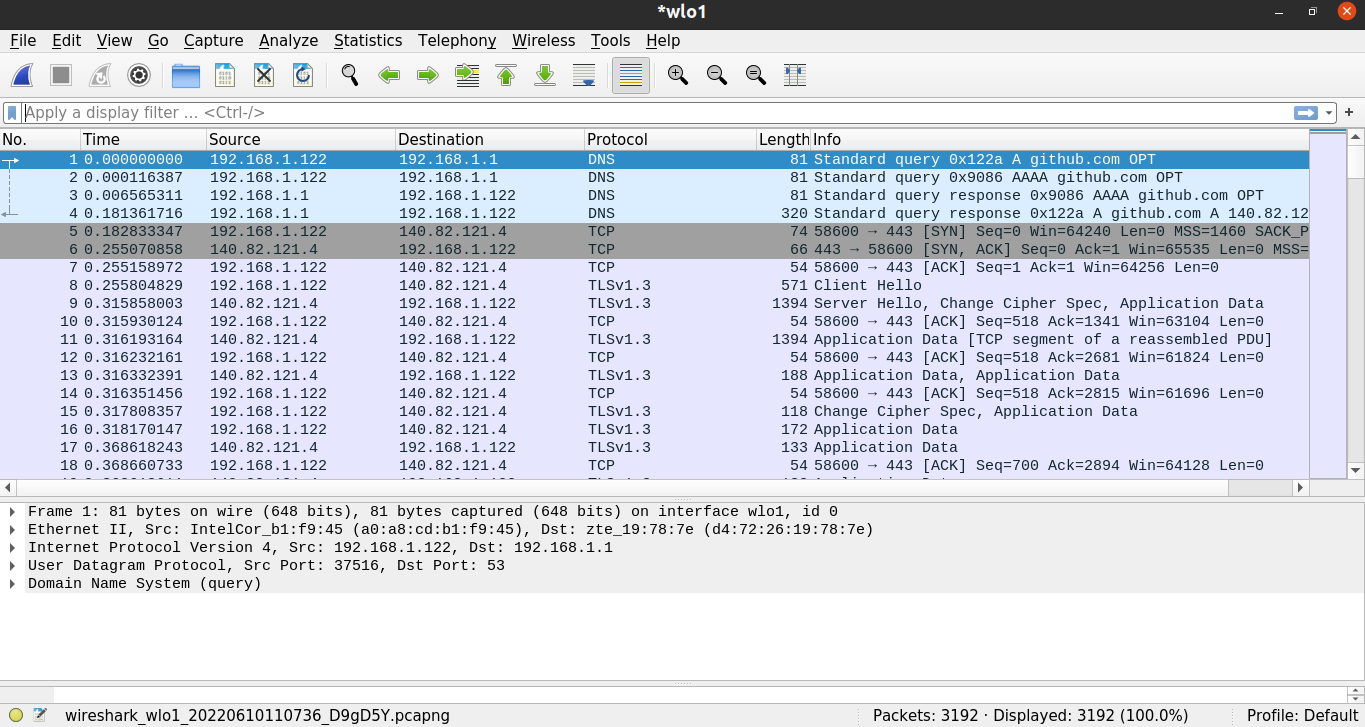
\includegraphics[scale=0.2]{h2load-wireshark}
\caption{captured during warmup time}
\label{fig:figure1}
\end{figure}


The packets were captured during the warmup phase of the command, which specifies 1 second of warmup time and 5 seconds for the duration of the actual benchmark:


h2load --warm-up-time 1 https://github.com --duration 5 


When warmup time is greater than 0, "time for connect" and "time to 1st byte" tend to become 0, as the following tables show:


\begin{table}[h!]
\centering
\begin{tabular}{|l|l|l|l|l|l|}
\hline
                  & min      & max      & mean     & sd   & +/- sd   \\ \hline
time for request: & 0us      & 0us      & 0us      & 0us  & 0.00\%   \\ \hline
time for connect: & 157.24ms & 157.24ms & 157.24ms & 0us  & 100.00\% \\ \hline
time to 1st byte: & 227.56ms & 227.56ms & 227.56ms & 0us  & 100.00\% \\ \hline
req/s             & 0.00     & 0.00     & 0.00     & 0.00 & 100.00\% \\ \hline
\end{tabular}

\caption{Without warmup time (warmup time = 0)}
\label{fig:table4}

\end{table}




\begin{table}[h!]
\centering
\begin{tabular}{|l|l|l|l|l|l|}
\hline
                  & min      & max      & mean     & sd      & +/- sd   \\ \hline
time for request: & 106.22ms & 164.90ms & 134.89ms & 14.35ms & 67.57\%  \\ \hline
time for connect: & 0us      & 0us      & 0us      & 0us     & 0.00\%   \\ \hline
time to 1st byte: & 0us      & 0us      & 0us      & 0us     & 0.00\%   \\ \hline
req/s             & 7.40     & 7.40     & 7.40     & 0.00    & 100.00\% \\ \hline
\end{tabular}

\caption{With warmup time = 1 second}
\label{fig:table5}

\end{table}


\subsection{Embedded Objects with nghttp}


Checking the Page Load Time of a website usually implies testing it out on a real browser; but nghttp, being a fully featured HTTP/2 client, supports downloading the embedded objects/assets of a web page, besides its html code, through the -a (--get-assets) option [\ref{article9}]. 


This means that it is possible to use nghttp to approximate the time that it would take for a real web browser to download the assets of a page from a web server. 

The following tables represent the behaviors of a website (https://archive.org) when downloaded using nghttp, with and without the -a flag:



\begin{table}[h!]
\centering
\begin{tabular}{|l|l|l|l|l|l|l|}
\hline
id & responseEnd & requestStart & process  & code & size & request path \\ \hline
13 & +308.00ms   & +175us       & 307.82ms & 200  & 1K   & /            \\ \hline

\end{tabular}

\caption{without the -a option}
\label{fig:table6}
\end{table}


\begin{table}[h!]
\centering

\resizebox{\columnwidth}{!}{%
\begin{tabular}{|l|l|l|l|l|l|l|}
\hline
id & responseEnd & requestStart & process  & code & size & request path                                                                          \\ \hline
13 & +408.96ms   & +151us       & 408.81ms & 200  & 1K   & /                                                                                     \\ \hline
15 & +717.76ms   & +409.29ms    & 308.47ms & 200  & 318K & /offshoot\_assets/index.56c7d2ac8e12.css                                              \\ \hline
17 & +717.97ms   & +409.30ms    & 308.67ms & 200  & 1K   & /offshoot\_assets/vendor/lit@2.0.2/polyfill-support.js                                \\ \hline
19 & +718.15ms   & +409.30ms    & 308.85ms & 200  & 1K   & /offshoot\_assets/vendor/@webcomponents/webcomponentsjs@2.6.0/webcomponents-loader.js \\ \hline
21 & +718.31ms   & +409.30ms    & 309.01ms & 200  & 2K   & /offshoot\_assets/js/webpack-runtime.278ae0d32b8bdea6e95a.js                          \\ \hline
23 & +1.95s      & +409.30ms    & 1.54s    & 200  & 103K & /offshoot\_assets/js/index.2d907721752dd736f0e5.js                                    \\ \hline


\end{tabular}%
}
\caption{with the -a option}
\label{fig:table7}
\end{table}


As one can see from the tables, the -a option can give a rough idea of the PLT of the page on an actual browser, keeping in mind that on an actual browser the "perceived" PLT will always be higher, as this kind of test doesn't take into account the time needed for the web engine to render the content and run the scripts.


% idk, latex just needs this here for bibliography linking to work properly:
\clearpage


\section{Conclusions}

The source code of this report, as well as that of the tests, and the data that was collected, is all available on the associated Github repository [\ref{article7}].


\section{References}

\begin{enumerate}

\item \label{article1} \url{https://www.hobo-web.co.uk/your-website-design-should-load-in-4-seconds/} 

\item \label{article2} \url{https://www.computerworld.com/article/2541429/hacking-firefox--the-secrets-of-about-config.html?page=5} 

\item \label{article3} \url{https://blog.stackpath.com/glossary-domain-sharding/} 

\item \label{article4} \url{https://httpd.apache.org/docs/2.4/programs/ab.html#synopsis} 

\item \label{article5} \url{https://developer.mozilla.org/en-US/docs/Web/HTTP/Caching} 

\item \label{article6} \url{http://manpages.ubuntu.com/manpages/trusty/man1/xdotool.1.html} 

\item \label{article7} \url{https://github.com/aiman-al-masoud/edi_reports} 

\item \label{article8} \url{https://nghttp2.org/documentation/h2load.1.html} 

\item \label{article9} \url{https://nghttp2.org/documentation/nghttp.1.html} 


\end{enumerate}

\end{document}
